\section{Equilibrio de Nash en el Juego Kunh Poker}

La descripción del juego se encuentra en la sección \ref{section:kuhn-poker}. Con respecto a la solución, se tiene que el jugador $2$ tiene una ganancia esperada de $\frac{1}{18}$ por mano, como se prueba en \cite{bib:kuhn-poker}, si ambos jugadores juegan de forma óptima (es decir, acorde a un equilibrio de Nash). El equilibrio de Nash se resume en la Tabla \ref{tab:estrategia-kuhn-poker}, donde los conjuntos de información fueron enumerados en un orden de búsqueda por profundidad (dfs).

\begin{table}[ht]
    \centering
    \begin{tabular}{c|r r}
        \hline
        I & \multicolumn{2}{|c}{Equilibrio de Nash}  \\ \hline
         $1$ & $1-\alpha$ & $\alpha$ \\
         $2, 3, 6, 10$ & $1$ & $0$ \\
         $4$ & $\frac{2}{3}$ & $\frac{1}{3}$ \\
         $5, 7, 12$ & $0$ & $1$ \\
         $8$ & $\frac{2}{3}$ & $\frac{1}{3}$ \\
         $9$ & $\frac{2}{3} - \alpha$ & $\alpha + \frac{1}{3}$ \\
        $11$ & $1 - 3 \alpha$ & $3 \alpha$ \\ \hline
    \end{tabular}
    \caption{Equilibrio de Nash para el juego de Kuhn Poker}
    \label{tab:estrategia-kuhn-poker}
\end{table}


El primer jugador tiene infinitas estrategias óptimas, las cuales pueden ser representadas por la elección de un parámetro $\alpha \in [ 0, \frac{1}{3} ]$. Una vez elegido este parámetro, el primer jugador en su primera jugada debe apostar con probabilidad $\alpha$ cuando su carta tenga el número $1$, apuestar con una probabilidad $3 \alpha$ cuando tenga el número $3$ y pasar siempre cuando tenga el número $2$. Si el primer jugador tiene un segundo turno, debe pasar siempre que tenga el número $1$, apostar cuando tiene el número $3$, y en el caso que tenga el número $2$ debe apostar con probabilidad $\alpha + \frac{1}{3}$.

El segundo jugador tiene una única estrategia mixta óptima: apostar siempre que tenga el número $3$. Cuando tenga el número $1$, pasar siempre que el primer jugador haya apostado y apostar con probabilidad $\frac{1}{3}$ en caso contrario. Cuando tenga el número $2$, debe pasar cuando el oponente haya pasado previamente y apostar con probabilidad $\frac{2}{3}$ en caso contrario. La figura \ref{fig:kunh-poker-estrategias} muestra el árbol con las distribuciones de probabilidad de las estrategias previamente descritas en cada uno de los nodos alcanzables en el juego.

\begin{figure}[ht]
\begin{center}
\caption{Equilibrio de Nash del juego de Kunh poker}
\label{fig:kunh-poker-estrategias}
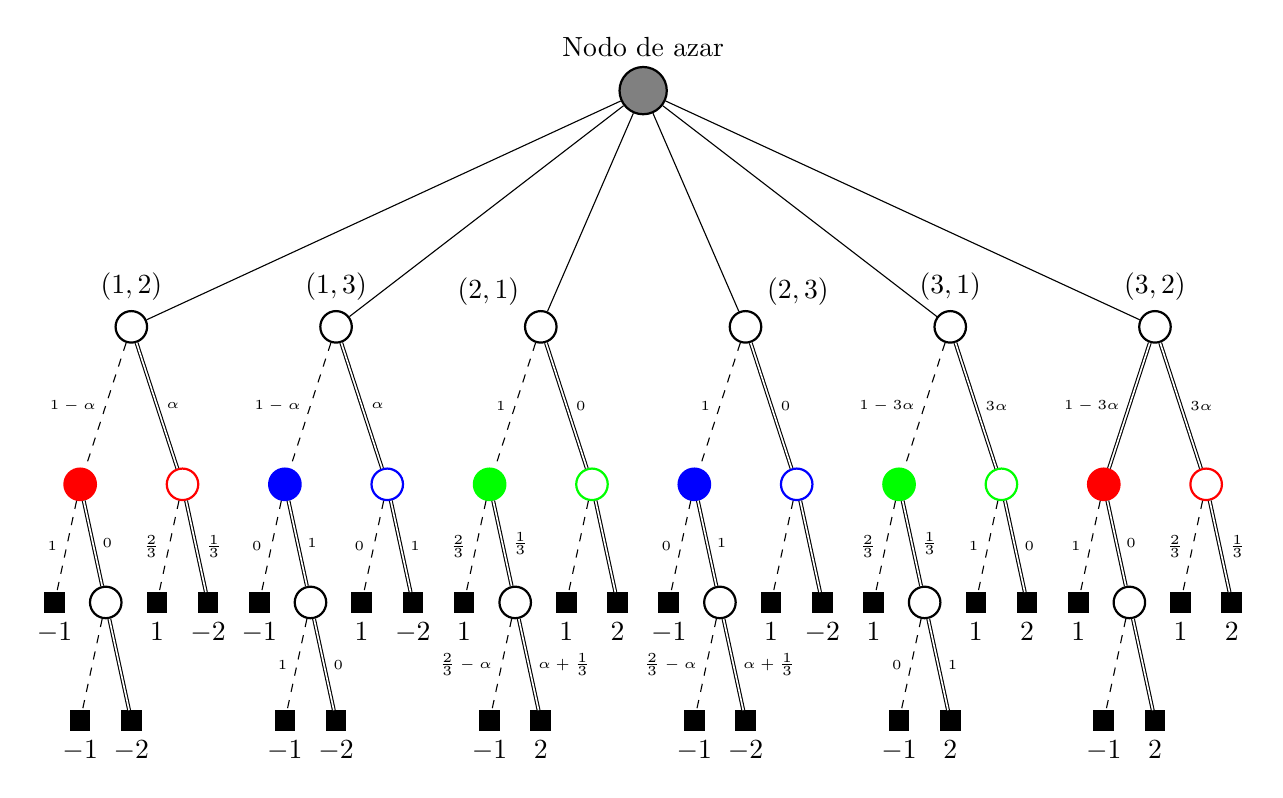
\begin{tikzpicture}[
chance/.style={circle, draw=black, fill=gray, thick, minimum size = 6mm},
player1/.style={circle, draw=black, solid, thick, minimum size = 4mm},
player2/.style={circle, thick, minimum size=4mm},
terminal/.style={rectangle, draw=black, solid, fill=black, thick, minimum size=2mm},
level 1/.style={sibling distance=26mm, level distance=30mm},
level 2/.style={sibling distance=13mm, level distance=20mm},
level 3/.style={sibling distance=6.5mm, level distance=15mm},
]
\node[chance] [label=above:{Nodo de azar}] {} {
	child {node [player1] (P1) [label=above:{$(1, 2)$}]{}
		child { node [player2] [draw=red, fill=red] {} 
				child { node [terminal] [label=below:{$-1$}] {}
						edge from parent [dashed] node [left, draw=none] {\tiny{$1$}} {} }
				child { node [player1] (A) {} 
						child { node [terminal] [label=below:{$-1$}] {}
								edge from parent [dashed] {} }
						child { node [terminal] [label=below:{$-2$}] {} 
								edge from parent [solid, double] {} }
						edge from parent [solid, double] node [right, draw=none] {\tiny{$0$}}  {}
				}
				edge from parent [dashed] node [left, draw=none] {\tiny{$1-\alpha$}}  {}
		}
		child { node [player2] [draw=red] {} 
				child { node [terminal] [label=below:{$1$}] {}
						edge from parent [dashed] node [left, draw=none] {\tiny{$\frac{2}{3}$}} {} }
				child { node [terminal] [label=below:{$-2$}] {}
						edge from parent [solid, double] node [right, draw=none] {\tiny{$\frac{1}{3}$}} {} }
				edge from parent [solid, double] node [right, draw=none] {\tiny{$\alpha$}}{}
		}
	}
	child {node [player1] (P2) [label=above:{$(1, 3)$}]{}
		child { node [player2] [draw=blue, fill=blue] {} 
				child { node [terminal] [label=below:{$-1$}] {}
						edge from parent [dashed] node [left, draw=none] {\tiny{$0$}} {} }
				child { node [player1] (B) {} 
						child { node [terminal] [label=below:{$-1$}] {}
								edge from parent [dashed] node [left, draw=none] {\tiny{$1$}} {} }
						child { node [terminal] [label=below:{$-2$}] {}
								edge from parent [solid, double] node [right, draw=none] {\tiny{$0$}} {} }
						edge from parent [solid, double] node [right, draw=none] {\tiny{$1$}} {}
				}
				edge from parent [dashed] node [left, draw=none] {\tiny{$1-\alpha$}} {}
		}
		child { node [player2] [draw=blue] {} 
				child { node [terminal] [label=below:{$1$}] {}
						edge from parent [dashed] node [left, draw=none] {\tiny{$0$}} {} }
				child { node [terminal] [label=below:{$-2$}] {}
						edge from parent [solid, double] node [right, draw=none] {\tiny{$1$}} {} }
				edge from parent [solid, double] node [right, draw=none] {\tiny{$\alpha$}} {}
		}
	}
	child {node [player1] (P3) [label=135:{$(2, 1)$}]{}
		child { node [player2] [draw=green, fill=green] {} 
				child { node [terminal] [label=below:{$1$}] {}
						edge from parent [dashed] node [left, draw=none] {\tiny{$\frac{2}{3}$}} {} }
				child { node [player1] (C) {} 
						child { node [terminal] [label=below:{$-1$}] {}
								edge from parent [dashed] node [left, draw=none] {\tiny{$\frac{2}{3}-\alpha$}} {} }
						child { node [terminal] [label=below:{$2$}] {} 
                        		edge from parent [solid, double] node [right, draw=none] {\tiny{$\alpha+\frac{1}{3}$}} {} }
						edge from parent [solid, double] node [right, draw=none] {\tiny{$\frac{1}{3}$}} {}
				}
				edge from parent [dashed] node [left, draw=none] {\tiny{$1$}} {}
		}
		child { node [player2] [draw=green] {} 
				child { node [terminal] [label=below:{$1$}] {}
						edge from parent [dashed] {} }
				child { node [terminal] [label=below:{$2$}] {}
						edge from parent [solid, double] {} }
				edge from parent [solid, double] node [right, draw=none] {\tiny{$0$}} {}
		}
	}
	child {node [player1] (P4) [label=45:{$(2, 3)$}]{}
		child { node [player2] [draw=blue, fill=blue]{} 
				child { node [terminal] [label=below:{$-1$}] {}
						edge from parent [dashed] node [left, draw=none] {\tiny{$0$}} {} }
				child { node [player1] (D) {} 
						child { node [terminal] [label=below:{$-1$}] {}
								edge from parent [dashed] node [left, draw=none] {\tiny{$\frac{2}{3}-\alpha$}} {} {} }
						child { node [terminal] [label=below:{$-2$}] {}
								edge from parent [solid, double] {} node [right, draw=none] {\tiny{$\alpha+\frac{1}{3}$}} {} }
						edge from parent [solid, double] node [right, draw=none] {\tiny{$1$}} {}
				}
				edge from parent [dashed] node [left, draw=none] {\tiny{$1$}} {}
		}
		child { node [player2] [draw=blue] {} 
				child { node [terminal] [label=below:{$1$}] {}
						edge from parent [dashed] {} }
				child { node [terminal] [label=below:{$-2$}] {}
						edge from parent [solid, double] {} }
				edge from parent [solid, double] node [right, draw=none] {\tiny{$0$}} {}
		}
	}
	child {node [player1] (P5) [label=above:{$(3, 1)$}]{}
		child { node [player2] [draw=green, fill=green] {} 
				child { node [terminal] [label=below:{$1$}] {}
						edge from parent [dashed] node [left, draw=none] {\tiny{$\frac{2}{3}$}} {} }
				child { node [player1] (E) {} 
						child { node [terminal] [label=below:{$-1$}] {}
								edge from parent [dashed] node [left, draw=none] {\tiny{$0$}} {} }
						child { node [terminal] [label=below:{$2$}] {}
								edge from parent [solid, double] node [right,draw=none] {\tiny{$1$}} {} }
						edge from parent [solid, double] node [right, draw=none] {\tiny{$\frac{1}{3}$}} {}
				}
				edge from parent [dashed] node [left, draw=none] {\tiny{$1-3 \alpha$}} {}
		}
		child { node [player2] [draw=green] {} 
				child { node [terminal] [label=below:{$1$}] {}
						edge from parent [dashed] node [left, draw=none] {\tiny{$1$}} {} }
				child { node [terminal] [label=below:{$2$}] {}
						edge from parent [solid, double] node [right, draw=none] {\tiny{$0$}} {} }
				edge from parent [solid, double] node [right, draw=none] {\tiny{$3 \alpha$}} {}
		}
	}
	child {node [player1] (P6) [label=above:{$(3, 2)$}]{}
		child { node [player2]  [draw=red, fill=red] {} 
				child { node [terminal] [label=below:{$1$}] {}
						edge from parent [dashed] node [left, draw=none] {\tiny{$1$}} {} }
				child { node [player1] (F) {} 
						child { node [terminal] [label=below:{$-1$}] {}
								edge from parent [dashed] {}}
						child { node [terminal] [label=below:{$2$}] {}
								edge from parent [solid, double] {} }
						edge from parent [solid, double] node [right, draw=none] {\tiny{$0$}} {}
				}
				edge from parent [solid, double] node [left, draw=none] {\tiny{$1-3\alpha$}} {}
		}
		child { node [player2]  [draw=red] {} 
				child { node [terminal] [label=below:{$1$}] {}
						edge from parent [dashed] node [left, draw=none] {\tiny{$\frac{2}{3}$}} {} }
				child { node [terminal] [label=below:{$2$}] {}
						edge from parent [solid, double] node [right, draw=none] {\tiny{$\frac{1}{3}$}} {} }
				edge from parent [solid, double] node [right, draw=none] {\tiny{$3\alpha$}} {}
		}
	}
};
\end{tikzpicture}
\end{center}
\end{figure}
